% Arch 4A --- Private angular centers + SB-LN (M15a)
% Compile: tectonic arch4a_angular_centers.tex
\documentclass[11pt]{article}
\usepackage[a4paper,landscape,margin=14mm]{geometry}
\usepackage{lmodern}
\usepackage{amsmath,amssymb}
\usepackage{xcolor}
\usepackage{array,booktabs}
\usepackage{tikz}
\usetikzlibrary{arrows.meta,positioning,fit,backgrounds,calc}
\pagestyle{empty}
\setlength{\parindent}{0pt}
\newcolumntype{L}[1]{>{\raggedright\arraybackslash}p{#1}}

\definecolor{box}{HTML}{EEF2F7}
\definecolor{trn}{HTML}{FCE9C8}
\definecolor{frz}{HTML}{DCE6F2}
\definecolor{prv}{HTML}{E3F1DF}
\definecolor{nov}{HTML}{F8E6EF}

\tikzset{
  blk/.style={draw,rounded corners=3pt,fill=box,align=center,font=\normalsize,minimum height=18mm,text width=46mm,line width=0.8pt},
  frz/.style={blk,fill=frz},
  trn/.style={blk,fill=trn},
  prv/.style={blk,fill=prv},
  nov/.style={blk,fill=nov},
  lab/.style={font=\footnotesize,text=black!80,inner sep=1.5pt},
  ar/.style={-{Latex[length=3mm]},line width=1.1pt}}

\begin{document}

\begin{center}
{\Large\bfseries Arch 4A --- Private Angular Centers + SB-LN (M15a)}\\[2pt]
{\small Orange = deployed trained; green = training-only private; blue = frozen. Avoids Arch~2/3 failure mode: private latent is \textbf{not} on LN values or a feature shift \(W\delta\).}
\end{center}
\vspace{3mm}

\begin{center}
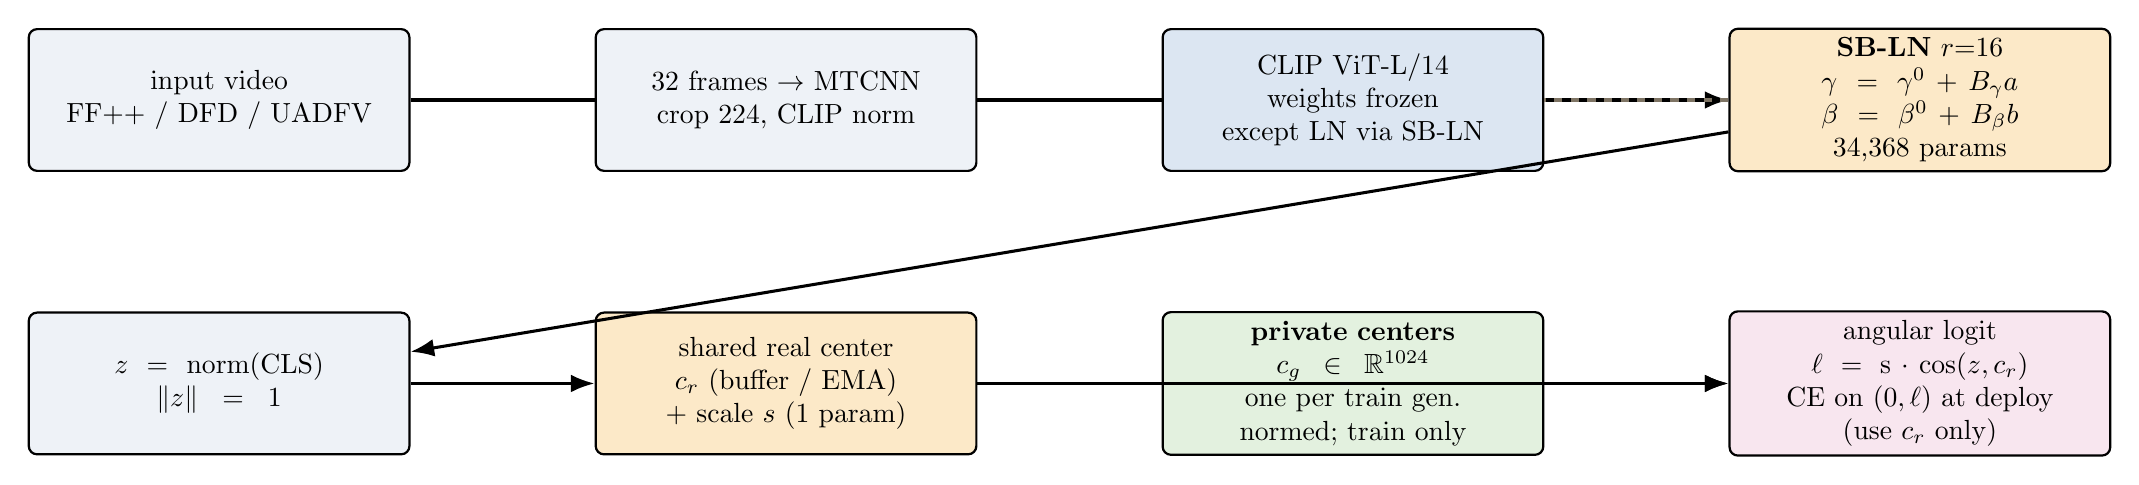
\begin{tikzpicture}[x=72mm,y=-36mm]
\node[blk] (vid) at (0,0) {input video\\FF++ / DFD / UADFV};
\node[blk] (pre) at (1,0) {32 frames $\to$ MTCNN\\crop $224$, CLIP norm};
\node[frz] (enc) at (2,0) {CLIP ViT-L/14\\weights frozen\\except LN via SB-LN};
\node[trn] (sb) at (3,0) {\textbf{SB-LN} $r{=}16$\\$\gamma=\gamma^0+B_\gamma a$\\$\beta=\beta^0+B_\beta b$\\34{,}368 params};
\node[blk] (z) at (0,1) {$z=\mathrm{norm}(\mathrm{CLS})$\\$\|z\|=1$};
\node[trn] (cr) at (1,1) {shared real center\\$c_r$ (buffer / EMA)\\+ scale $s$ (1 param)};
\node[prv] (cg) at (2,1) {\textbf{private centers}\\$c_g\in\mathbb{R}^{1024}$\\one per train gen.\\normed; train only};
\node[nov] (hd) at (3,1) {angular logit\\$\ell=\mathrm{s}\cdot\cos(z,c_r)$\\CE on $(0,\ell)$ at deploy\\(use $c_r$ only)};
\draw[ar] (vid)--(pre)--(enc)--(sb); \draw[ar] (sb)--(z);
\draw[ar] (z)--(cr); \draw[ar] (cr)--(hd); \draw[ar] (cg)--(hd);
\draw[line width=1.1pt,dashed,trn!50!black] (sb)--(enc);
\end{tikzpicture}
\end{center}

\vspace{4mm}
\begin{center}
{\normalsize\bfseries Training loss (private centers linked)}
\end{center}
\vspace{2mm}
\begin{center}
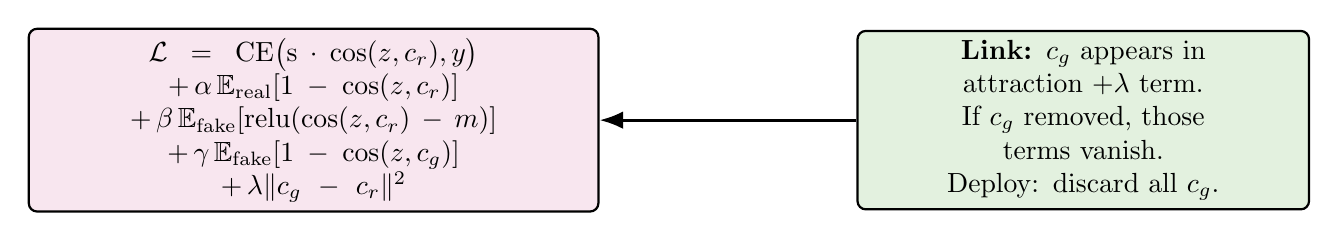
\begin{tikzpicture}[x=85mm,y=-32mm]
\node[nov,text width=70mm] (L) at (0,0)
 {$\mathcal{L}=\mathrm{CE}\big(\mathrm{s}\cdot\cos(z,c_r),y\big)$\\
  $+\,\alpha\,\mathbb{E}_{\mathrm{real}}[1-\cos(z,c_r)]$\\
  $+\,\beta\,\mathbb{E}_{\mathrm{fake}}[\mathrm{relu}(\cos(z,c_r)-m)]$\\
  $+\,\gamma\,\mathbb{E}_{\mathrm{fake}}[1-\cos(z,c_g)]$\\
  $+\,\lambda\|c_g-c_r\|^2$};
\node[prv,text width=55mm] (link) at (1.15,0)
 {\textbf{Link:} $c_g$ appears in\\attraction $+\lambda$ term.\\If $c_g$ removed, those\\terms vanish.\\Deploy: discard all $c_g$.};
\draw[ar] (link)--(L);
\end{tikzpicture}
\end{center}

\vspace{4mm}
\begin{center}
\small
\begin{tabular}{L{55mm}rrr}
\toprule
piece & count & deployed? \\
\midrule
SB-LN ($r{=}16$) & 34{,}368 & yes \\
scale $s$ (or $b,\tau$) & 1--2 & yes \\
private $c_g$ ($G{\times}1024$) & 4{,}096 & \textbf{no} \\
\textbf{deployed total} & $\approx$34{,}370 & \\
\textbf{train-time} & $\approx$38{,}466 & \\
\bottomrule
\end{tabular}
\hspace{8mm}
\begin{tabular}{L{70mm}L{70mm}}
\toprule
vs prior & difference \\
\midrule
Arch 1 GBLA & private on LN $\gamma,\beta$, linear head \\
Arch 3 & private $\delta_g$ via $W$ shift of $\mu_f$ \\
\textbf{Arch 4A} & private = \textbf{angular centers} in the loss \\
\bottomrule
\end{tabular}
\end{center}

\vfill
{\small Notebook: \texttt{M15a.ipynb}. Decision: KEEP iff NT $\ge$ A0 (81.21) and DFD $\ge95.5$. Four aims: (1) SB-LN+angular head not LN+linear; (2) angular+attraction loss; (3) $c_g$ in $\mathcal{L}$; (4) deployed $\ll104{,}450$.}

\newpage
% =====================================================================
% PAGE: Novelty we can claim for this pipeline
% =====================================================================
\begin{center}
{\Large\bfseries Novelty --- Arch 4A (Private Angular Centers)}\\[2pt]
{\small Design claims for this pipeline only. Accuracy status after M15a: \textbf{REJECT} (NT/DFD collapsed) --- do not claim empirical superiority.}
\end{center}
\vspace{4mm}

\small
\renewcommand{\arraystretch}{1.35}
\begin{tabular}{L{8mm}L{42mm}L{85mm}L{70mm}}
\toprule
\# & claim & what is new in \textbf{this} pipeline & vs closest prior (this project) \\
\midrule
N1 & \textbf{Angular shared head} & Deployed score is $s\cdot\cos(z,c_r)$ with one scale $s$; no $1024{\to}2$ linear head. & Arch~1 linear head (2{,}050); Arch~3 prototype midpoint head \\
N2 & \textbf{Private angular centers} & Per-generator $c_g\in\mathbb{R}^{1024}$ on the sphere; training-only; discarded at deploy. & Arch~1/2 LN-value $\delta$; Arch~3 feature $\delta$ via $W$ \\
N3 & \textbf{Center-linked loss} & $\gamma\,\mathbb{E}[1-\cos(z,c_g)]+\lambda\|c_g-c_r\|^2$ makes $\mathcal{L}$ depend on $c_g$ by construction. & Arch~3 PFAL to $c_f(W\delta)$; not center parameters themselves \\
N4 & \textbf{SB-LN compression} & Shared LN path $2{\cdot}1024r+100r$ ($\approx$34k at $r{=}16$). & Arch~1 full 102{,}400 LNs \\
N5 & \textbf{Train/deploy split} & Deploy SB-LN $+\,s\,+\,c_r$ only; private $c_g$ never used at test. & Same philosophy as GBLA; new private content \\
\bottomrule
\end{tabular}

\vspace{6mm}
\begin{center}
\begin{tabular}{L{50mm}L{120mm}}
\toprule
four aims & how 4A addresses them (design) \\
\midrule
1. Not LN + linear alone & SB-LN + angular head \\
2. New loss & CE on $s\cos$ + real-anchor + margin + attract-to-$c_g$ + $\lambda$ \\
3. Private $\leftrightarrow$ loss & $c_g$ in attraction and penalty terms \\
4. $P\lt104{,}450$ & deployed $\approx$34{,}369 \\
\bottomrule
\end{tabular}
\end{center}

\vfill
{\small\textbf{What not to claim after M15a:} state-of-the-art / KEEP under the pre-registered gate (seen $\approx$43, NT $\approx$46, DFD $\approx$45). Use 4A as a \emph{negative} ablation: private angular centers under SB-LN did not yield a usable detector.}

\end{document}
